\chapter{Testing and Evaluation}
\label{chap:eval}
\lhead{\emph{Project Testing}}
%The goal of this chapter is an objective evaluation of the final system. The evaluation must be quantitative and not qualitative. You may perform qualitative evaluation but this should not form the basis of the main conclusions you derive from the evaluation. This evaluation, where possible, should be comparative, i.e. you should evaluate your system against a commercially available system and/or system detailed in a research publication. You should demonstrate operational testing of the project using real or contrived data sets to evaluate aspects of the project not encompassed in the software testing (e.g. quantify how well does your project achieved the overall goal). 
%\begin{itemize}
%    \item For software based projects this will include, but should not be limited to, evaluation of non-functional requirements.
%    \item For infrastructural projects this testing should include system/network KPI analysis.
%    \item For analysis based projects (ML, malware or other) this may include model evaluation or YARA rule validation, for example.
%    \item For management projects, where software testing or infrastructure testing may not be in scope, the test process for the system is expected to be more rigorous and well described than a project incorporating significant development work.
%\end{itemize} 
%
%Some suggested sections (the nature of this chapter should be discussed in detail with your term 2 supervisor):
%
%\section{Metrics}
%Identify and describe the metrics you used to evaluate your project. You should have identified some of these in the research phase report but will detail these as you progress through the design.
%
%\section{System Testing}
%Describe the experimental setup for each metric, and how you obtained the measurements. Describe the inputs for each experiment
%
%\section{Results}
%Summarise the output data, and the statistical or other techniques to deduce your results. Summarise your results, including tables or graphs as appropriate with a brief description of each. here possible, compare your results with other products/systems. Identify any possible threats to the validity of your results, and discuss each briefly here (you will discuss in more detail in the next chapter).
%
This chapter will go into more detail into how DynamiCrypt actually works. There will various code snippets present throughout this chapter. After an explanation of how parts of the system work tests will also be carried out. 

\section{The Beginning}
C++ is a compiled language and DynamiCrypt requires quite a few libraries to be present for linking. The command to compile DynamiCrypt is the following.
\begin{lstlisting}
g++ *.cpp -lboost_system -lpthread -lboost_thread -lboost_program_options -lcryptopp -lpistache -o DynamiCrypt
\end{lstlisting}

\begin{figure}[!h]
  \centering
      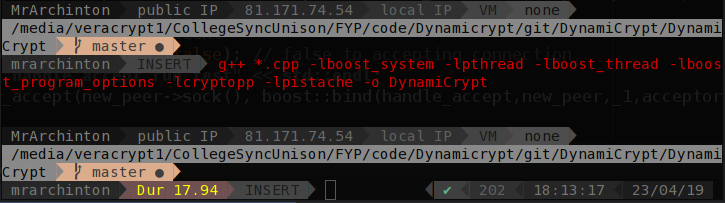
\includegraphics[width=1\textwidth]{Figures/b1.png}
  \caption[Compiling DynamiCrypt]{Compiling DynamiCrypt}
  \label{fig:b1}
\end{figure}
\FloatBarrier

Figure \ref{fig:b1} shows the result of the compilation and as you can see there are no errors or warnings present, this is an indication that the code is syntax correct and operations are performed for the correct data types.

Every program starts of with a main function. DynamiCrypt's main function is rather light, all it does is processes the command line arguments, creates a listening peer and creates the API server object.
To create an initial peer the already seen before code is used.
\begin{lstlisting}
ip::tcp::acceptor acceptor(service, ip::tcp::endpoint(ip::tcp::v4(), listen_port));
peer::ptr initial_peer = peer::new_(false);
acceptor.async_accept(initial_peer->sock(), boost::bind(handle_accept,initial_peer,_1, &acceptor));
\end{lstlisting}
Here an acceptor object is created this allows for the peer object to listen on a port on the localhost.
\begin{lstlisting}
peer::new_(false);
\end{lstlisting}
Is used to notify the peer object that this peer will be waiting for a connection.
\begin{lstlisting}
void handle_accept(peer::ptr peer, const boost::system::error_code & err, ip::tcp::acceptor* acceptor) {
    peer->start("",""); // starts current client
    // creates and listens for new client
    peer::ptr new_peer = peer::new_(false); // false to accepting connection
    //std::cout << "handle_accept run test" << std::endl;
    acceptor->async_accept(new_peer->sock(), boost::bind(handle_accept,new_peer,_1,acceptor)); // this 
}
\end{lstlisting}
The above function is called when the asynchronous connect object receives an external tcp request. The start method is called on the current peer followed by a creation of a new peer which will start listening for the next connection. This way there is always only one peer waiting for new connections. 

Because of how Boost manages asynchronous programming by using a service object to manage threads as well as using the proactor design pattern where asynchronous operations can occur using only one thread. However because DynamiCrypt is operation heavy when it comes to synchronisation I have used both threads and the proactor approach, this way when an asynchronous operation is about to take place Boost will choose a random available thread for it to run on. 
For this reason there are a few operations taking place in the main.cpp file to set all of this up.
\begin{lstlisting}
boost::thread_group threads;

start_listen(4);

void start_listen(int thread_count) {
    for ( int i = 0; i < thread_count; ++i)
        threads.create_thread( listen_thread);
}

void listen_thread() {
    service.run();
}

}
\end{lstlisting}
A group of threads variable is allocated, then the start listen function is called in the main function, this function creates four threads in this case and executes the service.run() function in each thread. This just executes boost asynchronous handler on each of the four threads. 

Finally to ensure a clean exit without leaving any zombie processes the main function will wait for all the threads to finish their execution.
\begin{lstlisting}
threads.join_all();
\end{lstlisting}

The API server is a bit more straight forward since the threads and asynchronous operations are more hidden away from the user by the Pistache library. 
\begin{lstlisting}
api_service_data_handler.set_address_and_port_of_sync("127.0.0.1", listen_port);
APIServer api_server(api_port);
\end{lstlisting}
The first line here sets the address of the sync-server and the port on which it is listening on as this information will be shared with the NodeJs app later. 
The actual creation of the API is simply calling the constructor with a port number.

The API and the sync-server require each other for operation, however it would be confusing if both were explained at the same time therefore the API will be covered initially followed by the sync-server.

\section{API}
The constructor of the API server creates the variables needed for the server and ofloads it to the APIservice object.
\begin{lstlisting}
APIServer::APIServer(int port_number) {
    Pistache::Port port(port_number);
    int thr = 2;
    Pistache::Address addr(Pistache::Ipv4::any(), port);
    //cout << "Cores = " << hardware_concurrency() << endl;
    std::cout << "API Using " << thr << " threads" << std::endl;
    API_service api(addr);
    api.init(thr);
    api.start();
    api.shutdown();
}
\end{lstlisting}
For the API two threads were defined as this is enough to handle multiple clients.
The threads are created as follows.
\begin{lstlisting}
void API_service::init(size_t thr = 2) {
    auto opts = Pistache::Http::Endpoint::options()
        .threads(thr)
        .flags(Pistache::Tcp::Options::InstallSignalHandler);
    httpEndpoint->init(opts);
    createDescription();
}
\end{lstlisting}
Pistache is a much more high level library than Boost therefore for the setup I mostly followed the examples they have in their GitHub repository.
\begin{lstlisting}
void API_service::start() {
    router.initFromDescription(desc);
    httpEndpoint->setHandler(router.handler());
    httpEndpoint->serve();
}
\end{lstlisting}
start() sets up the description which in Pistache's case is the information about all the routes available, some licensing and API info.  

Here is a small extract from the function that creates the description
\begin{lstlisting}
void API_service::createDescription() {
    desc
        .info()
        .license("Apache", "http://www.apache.org/licenses/LICENSE-2.0");

    auto backendErrorResponse =
        desc.response(Pistache::Http::Code::Internal_Server_Error, "An error occured with the backend");

    desc
        .schemes(Pistache::Rest::Scheme::Http)
        .basePath("/v1")
        .produces(MIME(Application, Json))
        .consumes(MIME(Application, Json));

    auto versionPath = desc.path("/v1");

    auto path = versionPath.path("/options");

    path
        .route(desc.get("/test-ok"))
        .bind(&API_service::route_test, this)
        .produces(MIME(Application, Json), MIME(Application, Xml))
        .response(Pistache::Http::Code::Ok, "ok");
    
    path
        .route(desc.post("/init"), "Initiate Communication")
        .bind(&API_service::initial, this)
        .produces(MIME(Application, Json))
        .consumes(MIME(Application, Json))
        .response(Pistache::Http::Code::Ok, "Initial request")
        .response(backendErrorResponse);
\end{lstlisting}
The path is built by firstly specifying the version of the API this way it is possible to support legacy code using you old API. Next I decided to put all the DynamiCrypt operations preceded by /options this way in the future if the API can be expanded to do other things like maybe formatting / encoding data. Next is the actual routes used by the DynamiCrypt API. The first one is /test-ok a GET route, this is handy if you want to check if the API is up and running. To access this route you would send a get request to this for example 127.0.0.1:9081/v1/options/test-ok/. This simple route will just return "ok" as can be seen when a curl get request is being made as can be seen in figure \ref{fig:b2}.

\begin{figure}[!h]
  \centering
      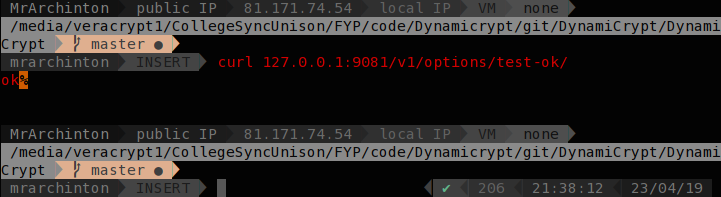
\includegraphics[width=1\textwidth]{Figures/b2.png}
  \caption[127.0.0.1:9081/v1/options/test-ok/]{127.0.0.1:9081/v1/options/test-ok/}
  \label{fig:b2}
\end{figure}
\FloatBarrier

The list of all routes currently available in the API and a brief description are as follows.
\begin{lstlisting}
/v1/options/test-ok         GET
// test if API is up
/v1/options/init            POST
// Initial request
/v1/options/init_config     POST
// Initial Config
/v1/options/sync            POST
// Begin Sync
/v1/options/status          POST
// check if connected to tpm ok
/v1/options/encrypt         POST
// encrypt / decrypt data
/v1/options/exit            POST
// delete tpm and data associated with the app using the API
/v1/options/:rest           POST
// custom 404
\end{lstlisting}

Every post route is handled by a specific function.
\begin{lstlisting}
 path
        .route(desc.post("/init"), "Initiate Communication")
        .bind(&API_service::initial, this)
        .produces(MIME(Application, Json))
        .consumes(MIME(Application, Json))
        .response(Pistache::Http::Code::Ok, "Initial request")
        .response(backendErrorResponse);
\end{lstlisting}

In this case every time the init route is called the initial() function handles it and produces its own response. Here is the initial function bellow.

\begin{lstlisting}
void API_service::initial(const Pistache::Rest::Request& request, Pistache::Http::ResponseWriter response) {
    rapidjson::Document document;
    // make into json object
    char * jsonBody = new char [request.body().length()+1];
    strcpy (jsonBody, request.body().c_str());
    document.Parse(jsonBody);
    
    std::string service_name;
    int data_ok = 1;

    if(document.HasMember("service_name")){
        if(document["service_name"].IsString()){
            service_name = document["service_name"].GetString();
        }
        else{
            data_ok = 0;
        }
    }
    else{
        data_ok = 0;
    }
    
    std::string respond_service_name;
    rapidjson::StringBuffer buffera;
    rapidjson::Writer<rapidjson::StringBuffer> writera(buffera);
    
    if(data_ok){
        respond_service_name = api_service_data_handler.new_service(service_name);
        writera.StartObject(); 
        writera.Key("service_name");                
        writera.String(respond_service_name.c_str(), respond_service_name.length());
        writera.Key("address_of_this_tpm");                
        writera.String(api_service_data_handler.get_sync_address().c_str(), api_service_data_handler.get_sync_address().length());
        writera.Key("port_of_this_tpm");
        writera.Uint(api_service_data_handler.get_sync_port());
        writera.EndObject();
        
    }
    
    else{//error with request
        writera.StartObject(); 
        writera.Key("error");                
        writera.String("invalid request");
        writera.EndObject();
    }
    
    response.send(Pistache::Http::Code::Ok, buffera.GetString());
}
\end{lstlisting}

Similar to NodeJs each of these handlers have a reference to a request and response object.
For extracting JSON data the RapidJson library is used, it is also used for creating JSON data.
The API interacts with the 
\begin{lstlisting}
api_service_data_handler
\end{lstlisting} 
object for managing the services.

It will take too long to go through all of the routes and how they function so a more basic explanation will suffice. I would recommend watching my demo video here https://www.youtube.com/watch?v=LsR4XsGrDCY&feature=youtu.be 
on YouTube as it would be easier to understand.

Initially the NodeJs apps must register with the API this unfortunately turned out to be a multi step process however it is necessary since the API needs data from both of the Apps that wish to use DynamiCrypt.

\begin{figure}[!h]
  \centering
      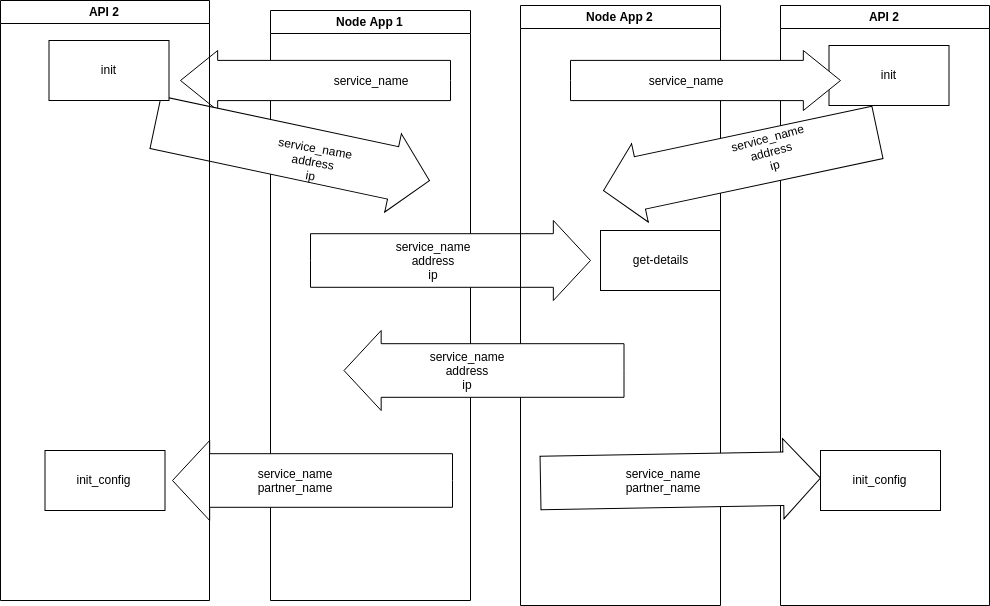
\includegraphics[width=1\textwidth]{Figures/connect_code_flow.png}
  \caption[How Node Apps register with the API]{How Node Apps register with the API}
  \label{fig:b3}
\end{figure}
\FloatBarrier

Figure \ref{fig:b3} is a call flow diagram of how the NodeJS apps register themselves with the API.
The same can be demonstrated by using Wireshark and listening on localhost. The filters I used are (tcp.port == 9081) && http since I only want to see POST requests for the API running on port 9081 since the POST requests for the other API are identical so there is no point in showing it twice.

\begin{figure}[!h]
  \centering
      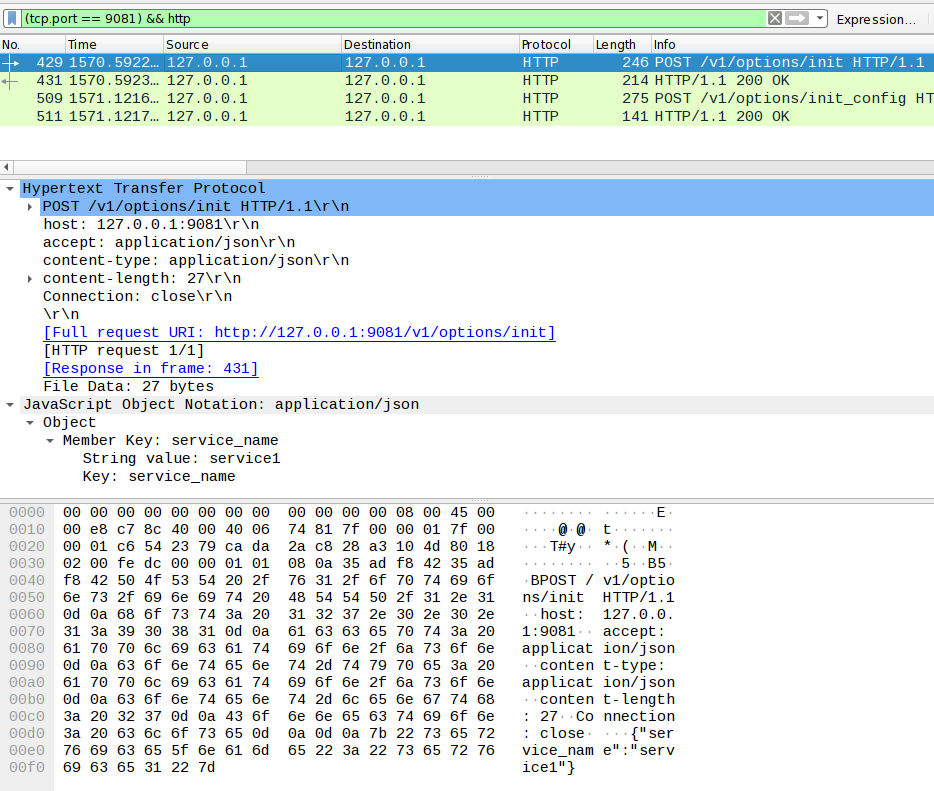
\includegraphics[width=1\textwidth]{Figures/b4.png}
  \caption[POST request to init]{POST request to init}
  \label{fig:b4}
\end{figure}
\FloatBarrier
Figure \ref{fig:b4} shows how the NodeJs App sent a POST request to the init route with its user service name. 

\begin{figure}[!h]
  \centering
      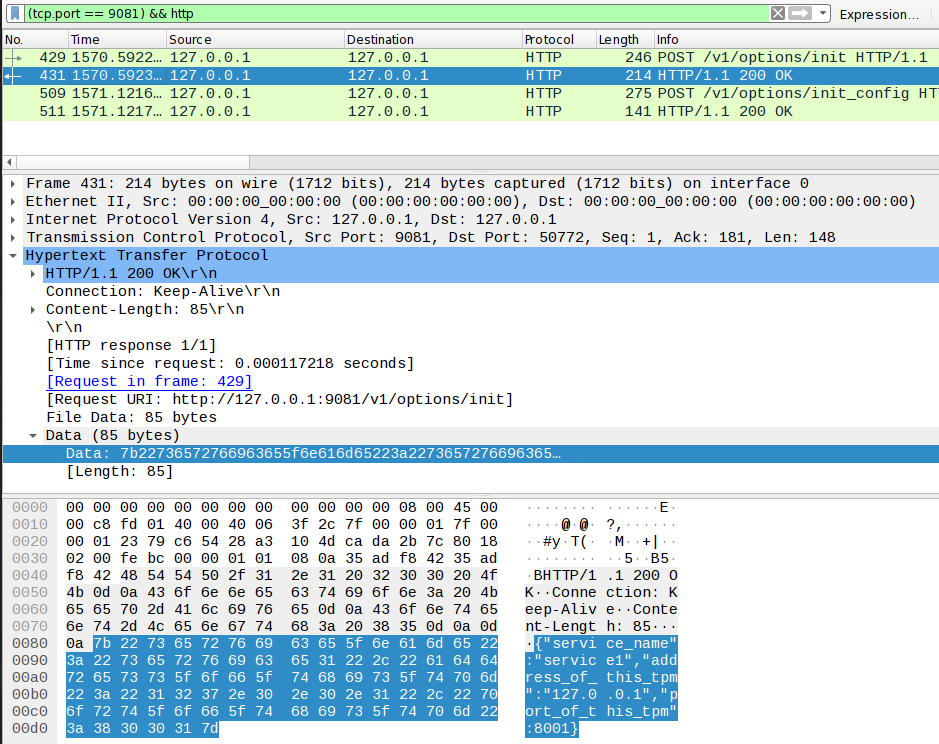
\includegraphics[width=1\textwidth]{Figures/b5.png}
  \caption[API response]{API response}
  \label{fig:b5}
\end{figure}
\FloatBarrier
Figure \ref{fig:b5} shows how the APIs reply to the previous post request with the service name the API wants the NodeJS App to use, the port of the sync-server and the address of the sync-server.
After this the Node App would make a request to the other Node App for the get details route to exchange information. This can also be acquired with Wireshark by changing a filter as seen in figure \ref{fig:b8}.
\begin{figure}[!h]
  \centering
      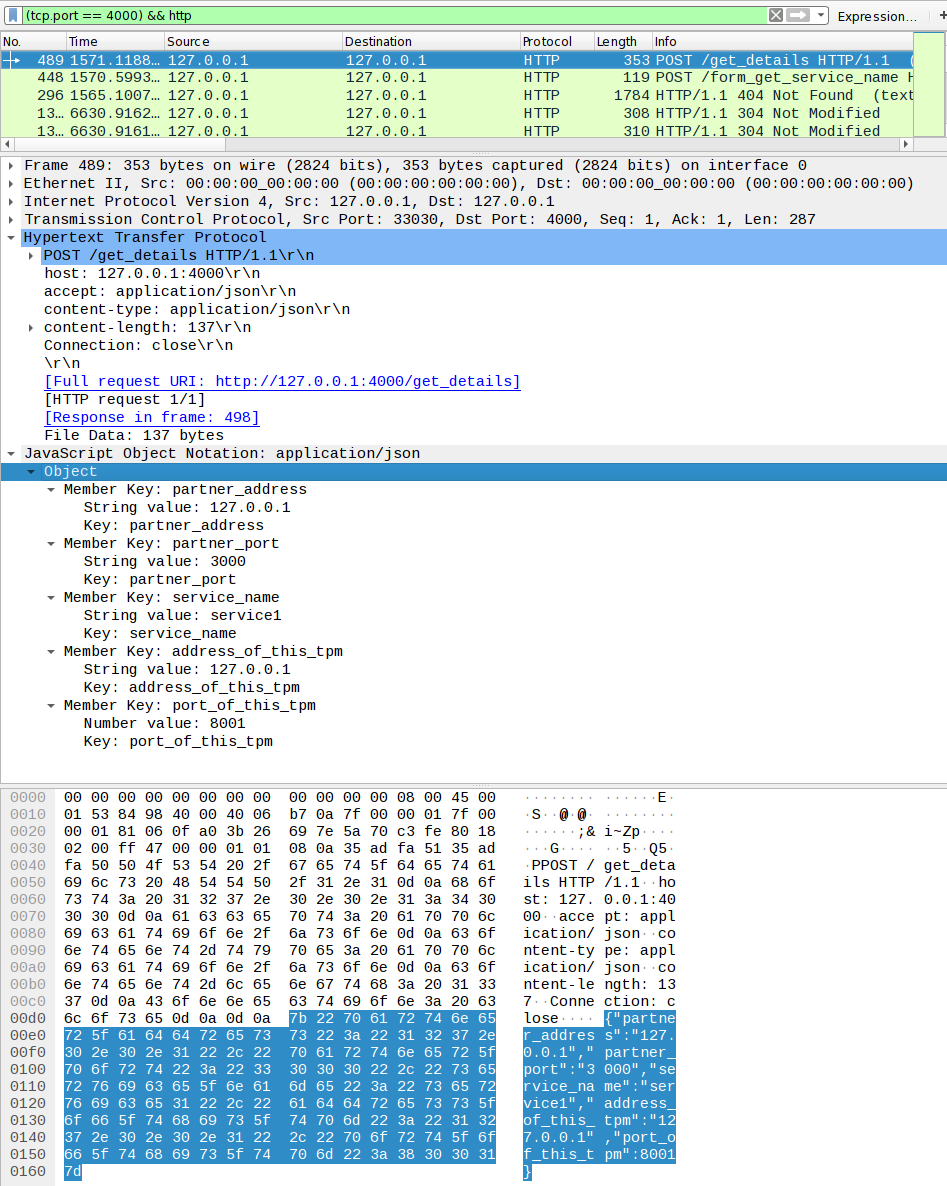
\includegraphics[width=1\textwidth]{Figures/b8.png}
  \caption[POST request to other NodeJs app's get details route]{POST request to other NodeJs app's get details route}
  \label{fig:b8}
\end{figure}
\FloatBarrier


\begin{figure}[!h]
  \centering
      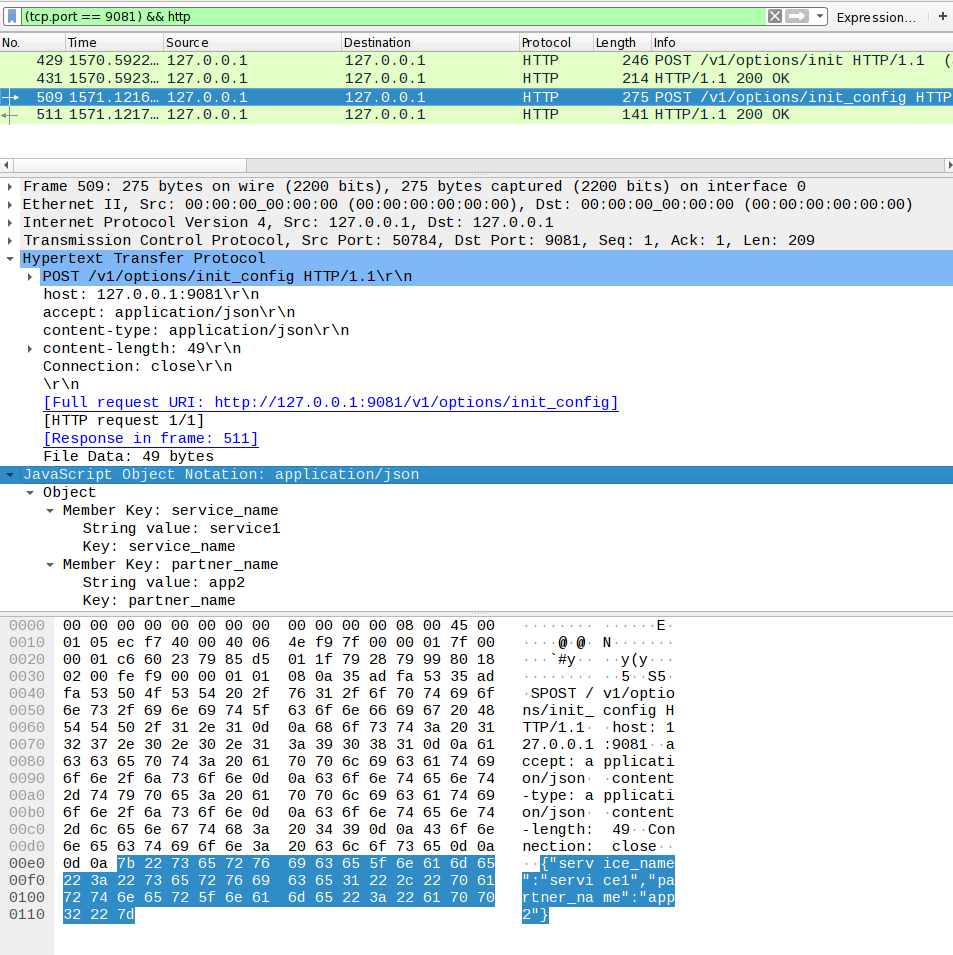
\includegraphics[width=1\textwidth]{Figures/b6.png}
  \caption[POST request to init config]{POST request to init config}
  \label{fig:b6}
\end{figure}
\FloatBarrier
Figure \ref{fig:b6} shows how the NodeJs app updates the API with the service name of the other NodeJs app in this case it is called partner name.

\begin{figure}[!h]
  \centering
      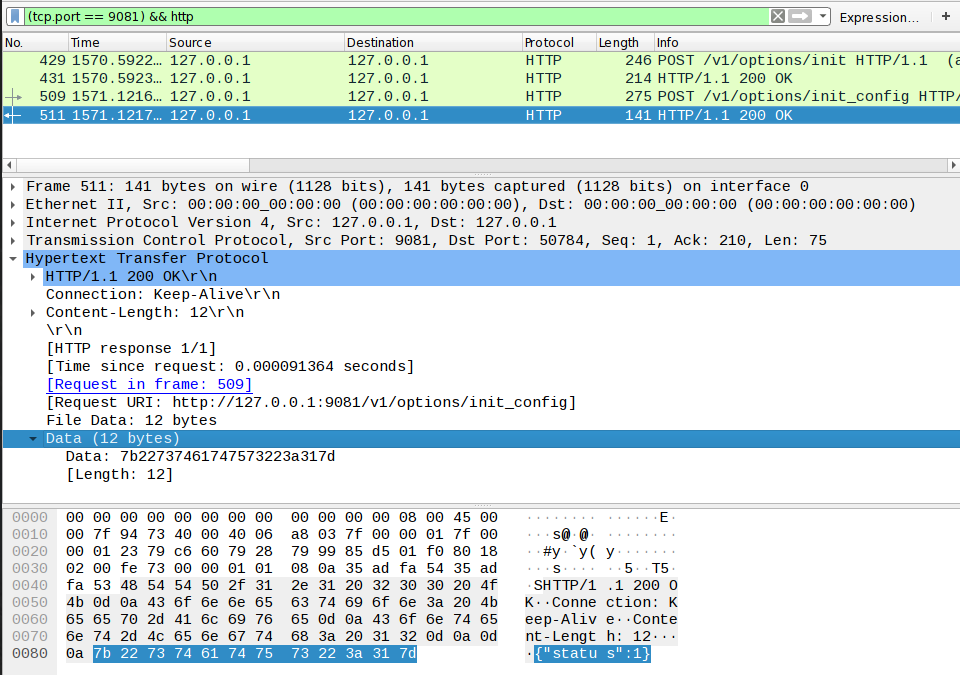
\includegraphics[width=1\textwidth]{Figures/b7.png}
  \caption[API response]{API response}
  \label{fig:b7}
\end{figure}
\FloatBarrier
Figure \ref{fig:b7} shows the APIs reply to the previous post request with a status 1 which means everything is OK and the update was successfully made.
Now the two NodeJs apps are fully registered with the API. The next step is to tell the API to tell the sync-server to start synchronising so that the Apps can send messages to each other using dynamic encryption.
For this to occur one of the Apps must simply call the sync route of the API.

\begin{figure}[!h]
  \centering
      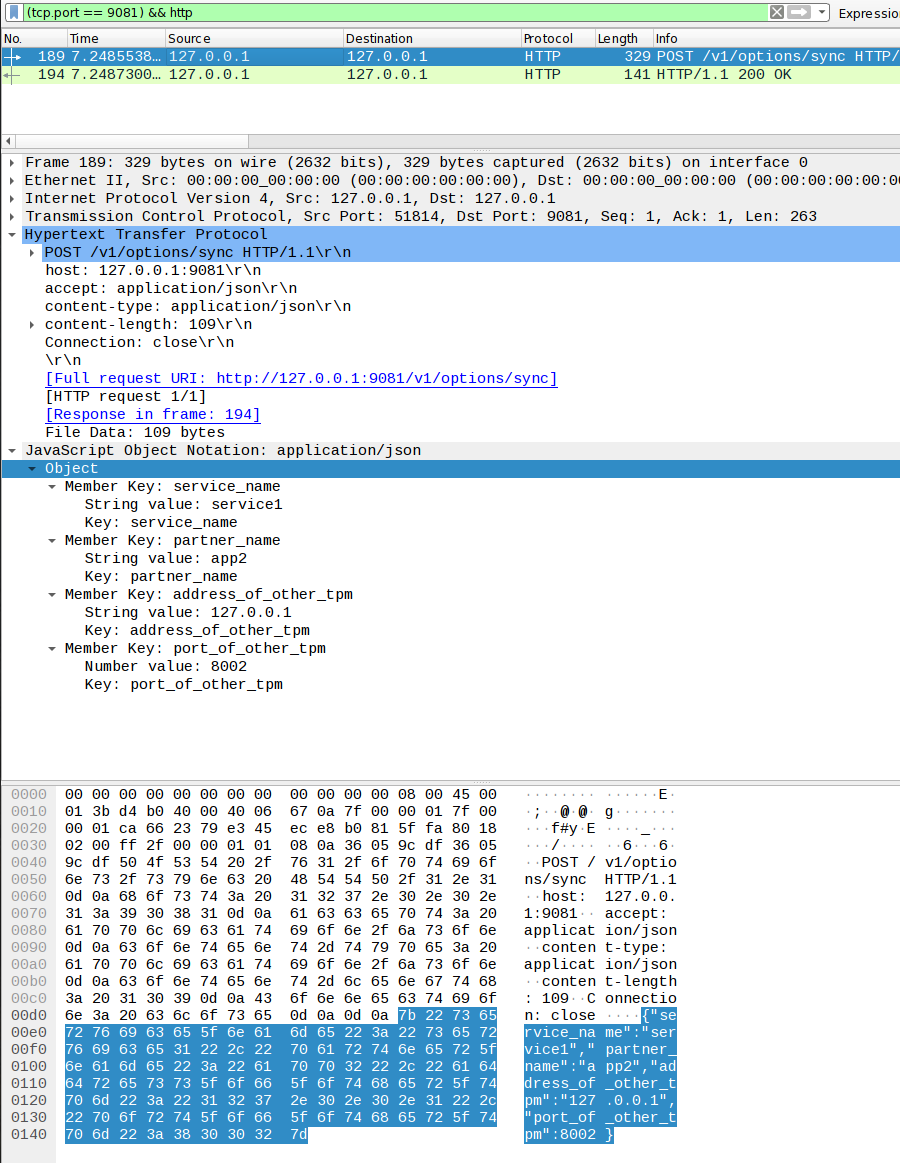
\includegraphics[width=1\textwidth]{Figures/b9.png}
  \caption[POST request to sync]{POST request to sync}
  \label{fig:b9}
\end{figure}
\FloatBarrier
Figure \ref{fig:b9} shows the sync route of the API is called. The Node App sends a lot of details this time including service name, partner name, the address and port of the sync-server that is used by the other API that the other NodeJs App communicates with. This is because it is calling a different function outside of the api service data handler object. This time a function from the definitions.cpp is called.
\begin{lstlisting}
int begin_sync(std::string address, int port, std::string service_name, std::string partner_name){
    try{
        peer::ptr initiating_peer = peer::new_(true, address, port);
        initiating_peer->start(service_name, partner_name);
    }
    catch(std::exception& e){
        return 0;
    }
    return 1;
}
\end{lstlisting} 
Here a new peer is created of connecting type instead of listening type like we looked at last time. This peer will try to connect to the sync-server at the address and port the Node App sent it.

\begin{figure}[!h]
  \centering
      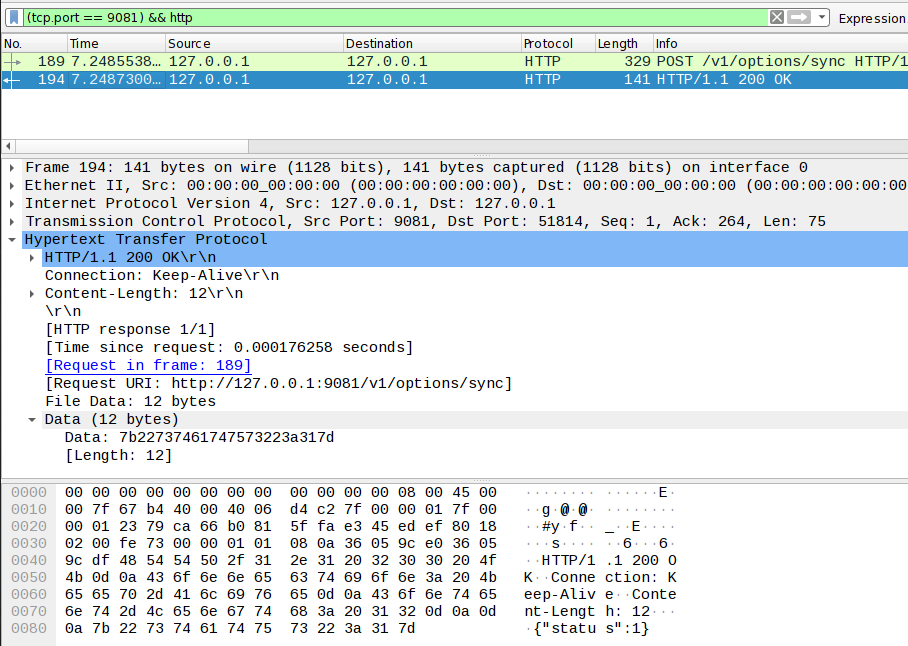
\includegraphics[width=1\textwidth]{Figures/b10.png}
  \caption[API response]{API response}
  \label{fig:b10}
\end{figure}
\FloatBarrier
Figure \ref{fig:b10} shows the APIs reply to the previous post request with a status 1 which means the request was processed successfully however this does not mean that the sync-server connected to the other sync-server correctly this is because of the asynchronous nature of the sync-server it is impossible to get the result of the connection. Therefore the NodeJs app should query the API to see if the connection was successful and if the two sync-servers are currently syncing this is done by calling the status route in the API and providing the service name. if the status returned is 1 then the two sync-servers are currently synchronising, if the status is 0 then they failed to connect or some other error occurred.

